\section{Methodology}\label{sect:methodology}
To address the challenges identified in~\cref{sect:related-work}, namely
evaluation-speed and categorization of near-classes, recent advances in machine
learning are considered. Contrary to most approaches in the field which perform
segmentation, this work focuses on detecting \glspl{bbox}. In this section,
details on the applied method is provided. Methods for object detection can coarsely
be divided into two groups: one-staged and two-staged approaches. To reduce complexity,
only a single one-stage approach will be considered in this paper. For details on
two stage detectors confer e.g.\ \cite{Ren.2015}.

\bigskip
{\large{\textbf{Single Shot MultiBox Detector}}}\\
Two common one-stage architectures are
\gls{yolo}~\cite{Redmon.2015, Redmon.2016b, Redmon.2018} and
\gls{ssd}~\cite{Liu.2016}. While \gls{ssd} can be extended to any base network
(e.g. VGG16~\cite{Simonyan.2015}), \gls{yolo} is limited to only Darknet~\cite{Redmon.2016}.
Therefore, \gls{ssd} was chosen over \gls{yolo} for this paper, retaining the
ability to quickly exchange base networks.

Central concepts of \gls{ssd} are described in the following.

\subsection{Default Boxes}\label{subsect:default-boxes}
The most fundamental part of understanding \gls{ssd} is understanding its specific
concept of \glspl{bbox}, default boxes and anchors. In order to reduce the very high
complexity, this subsection is written in a slightly more colloquial manner.

Slightly anticipating and simplifying \cref{subsect:SSD Architecture}, a
\emph{prediction} from \gls{ssd} is the output from a set of \glspl{convolutional layer}
that is chosen from within the network. Output of a single such \gls{layer} is,
first and foremost, just a \gls{feature map} --- while the goal is to find the
coordinates of a \gls{bbox} (and class predictions). 

Consider such a \gls{feature map} with dimensions \(m \times n\). Every pixel
from that \gls{feature map} contains highly condensed information about a specific
region from the original image\footnote{This concept is called the
\emph{receptive field} of \glspl{cnn}, \cite[cf.][331\psq]{Goodfellow.2016}}.
The \gls{feature map} is then processed further, s.t.\ for every such
pixel (and therefore the related region within the original image) receive the
coordinates of a single \gls{bbox} are received (simplified, for details see \cref{subsect:SSD Architecture}).

To the reader, this might be confusing. Receiving \(m\times n\)
single \gls{bbox} predictions for every pixel within the \gls{feature map} for
every chosen layer makes the number of predicted \glspl{bbox} \(\gg\) than the
expected number of \gls{gt} \glspl{bbox}. And it raises a pressing question:\linebreak
\textbf{How is training data constructed for such an unusual architecture?}

This question is answered (partly) by the introduction of \textbf{anchors}.

\paragraph{Anchors}\label{par:anchors}
Every pixel from a \gls{feature map} is related to a region within the original
input image (\emph{receptive field}~\cite[cf.][331\psq]{Goodfellow.2016}).
Furthermore, \glspl{convolutional layer} preserve the spatial structure of a
convolved image~\cite[cf.][335\psqq]{Goodfellow.2016}.

Therefore, every \emph{pixel} from within the feature map can be related
(very easily) to a region within the original image. The center of such region
is called the \textbf{anchor}. The x and y coordinates for every pixel \(p_{ij}\)
can then be calculated using \cref{eq:anch-x,eq:anch-y}. A practical example for an
image \(I\) of height and width \(I_w\times I_h=300\times 300\) and a
\gls{feature map} \(M\) of height and width \(M_w\times M_h=19\times 19\)
is shown in \cref{fig:vgg16-anchors}.

\begin{align}
    x_i&=0.5*\frac{w_I}{w_M} + \sum_{0}^{i-1} \frac{w_I}{w_M}\label{eq:anch-x}\\
    y_j&=0.5*\frac{h_I}{h_M} + \sum_{0}^{j-1} \frac{h_I}{h_M}\label{eq:anch-y}
\end{align}
where:
\begin{conditions}
    x_i & := & x-coordinates of the anchor for pixel \(p_{ij}\)\\
    y_j & := & y-coordinates of the anchor for pixel \(p_{ij}\)\\
    w_I & := & width of input image \(I\)\\
    w_M & := & width of feature map \(M\)\\
    h_I & := & height of input image \(I\)\\
    h_M & := & height of feature map \(M\)
\end{conditions}
\begin{figure}[t!]
    \centering
    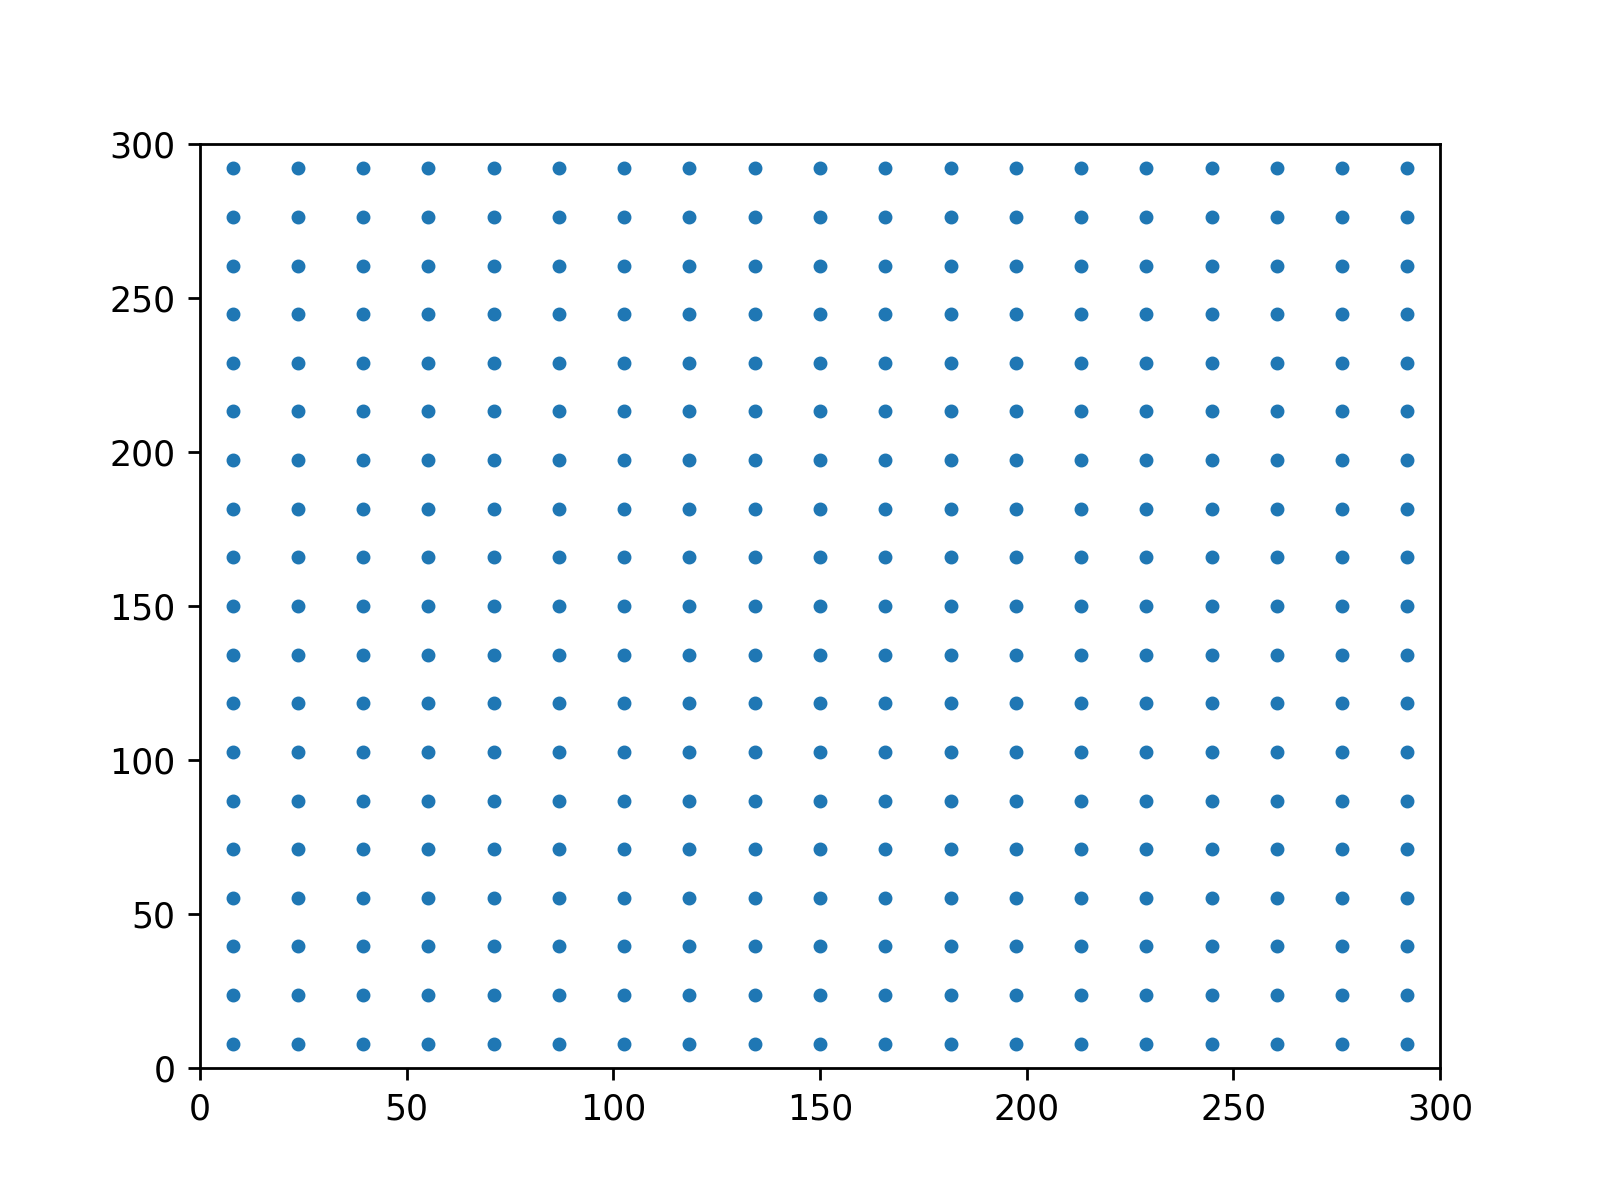
\includegraphics[width=0.5\textwidth]{vgg16-19x19}
    \caption{Generated anchors (blue) for an image of dimensions \(300\times 300\)
    and \gls{feature map} of \(19\times 19\).}\label{fig:vgg16-anchors}
\end{figure}
Now, training data could be constructed by assigning every \gls{gt} \gls{bbox} to
its closest anchor (from every chosen layer). An example of this is given in
\cref{eq:train-anchor}. 
\begin{equation}\label{eq:train-anchor}
    \begin{matrix}
        \ldots\\
        \begin{bmatrix}
            \ldots & \ldots & \ldots & \ldots & \ldots\\
            0 & 0 & 0 & 0 & 0\\
            271 & 828 & 182 & 845 & 1\\
            0 & 0 & 0 & 0 & 0\\
            \ldots & \ldots & \ldots & \ldots & \ldots
        \end{bmatrix}\\
        \ldots\\
        \begin{bmatrix}
            \ldots & \ldots & \ldots & \ldots & \ldots\\
            0 & 0 & 0 & 0 & 0\\
            3141 & 592 & 653 & 59 & 1\\
            0 & 0 & 0 & 0 & 0\\
            \ldots & \ldots & \ldots & \ldots & \ldots
        \end{bmatrix}\\
        \ldots
    \end{matrix}
\end{equation}
where the first four rows are x- and y-coordinate, height and width of the respective
\gls{bbox} and the last row is the class (0: \textit{no-object}, 1: \textit{object}).

This approach is flawed in two ways:
\begin{enumerate}
    \item Assigning \gls{gt} \glspl{bbox} to the closest anchor is entirely agnostic
    of the expected size of the receptive field for the different layers. A layer
    with smaller receptive field per pixel would probably not be able to perceive
    larger objects, while a layer with a larger receptive field might overlook
    smaller objects.\label{itm:anchor-flaw1}
    \item The model has no \textit{a priori} knowledge of \emph{position}, of
    \emph{x-} and \emph{y-coordinates}, of \emph{width} and \emph{height}.
    This is especially critical for images with different resolutions.\label{itm:anchor-flaw2}
\end{enumerate}
A possible solution to these flaws are \textbf{default boxes}.

\paragraph{Default Boxes}\label{par:default-boxes}
Default boxes are used to assign spatial representation to anchors. With such a
representation, every \gls{gt} \gls{bbox} can be matched to a set of anchors
more precisely (by overlap\footnote{The overlap could then be computed via
\gls{iou} for example --- as is done in \cref{eq:bbox-matcher}.} with respective
default boxes).

As a starting point, so far a set of chosen layers \(\mathbf{L} = \left\{L_0, L_1, \ldots, L_{n-1}\right\}\)
and a set of anchors for every such layer\footnotemark{} \(\mathbf{A} = \left\{A_0, A_1, \ldots, A_{n-1}\right\}\)
were constructed.

\footnotetext{More precisely, a set of anchors for the \glspl{feature map} produced
by such layer.}

Now, although the exact receptive fields of the chosen \glspl{layer} are uncertain,
their sizes, \(\abs*{recept\left(L\right)}\), \emph{are} known to be strictly
increasing with subsequent layers, i.e.\ \(\abs*{recept\left(L_0\right)} < \ldots < \abs*{recept\left(L_{n-1}\right)}\).

Fortunately, \textcite{Liu.2016} claim that the exact size of the receptive field is of
subordinate importance. Instead of calculating the exact receptive field, they
propose to assign a fixed edge length \(s_k\) for every chosen \gls{layer} per \cref{eq:default-box-size}:
\begin{equation}\label{eq:default-box-size}
    s_k=s_{_\text{min}} + k * \frac{s_{_\text{max}}-s_{_\text{min}}}{n-1}
\end{equation}
where:
\begin{conditions}
    n               &:= & \(\alphaAbs{L}\)\\
    k               &\in & [0, n-1]\\
    s_{_\text{min}} &=& 0.2\\
    s_{_\text{max}} &=& 0.9
\end{conditions}
A default box \(d_{i,j}\) for a pixel \(p_{i,j}\) within a given layer \(L_k\)
can then be computed as given in \cref{eq:dbox} (with h: height, w: width, x:
x-coordinate of the box's center, y: y-coordinate of the box's center).
\begin{align}
    \begin{split}\label{eq:dbox}
        d_{i,j}^h   &= s_k * h_I\\
        d_{i,j}^w   &= s_k * w_I\\
        d_{i,j}^x   &= x_i \text{ (see \cref{eq:anch-x})}\\
        d_{i,j}^y   &= y_j \text{ (see \cref{eq:anch-y})}
    \end{split}
\end{align}
It is now possible to match every \gls{gt} \gls{bbox} to a set of default boxes
per \cref{eq:bbox-matcher}.
\begin{equation}\label{eq:bbox-matcher}
    match(b, d) =
    \begin{cases}
        1 & \text{if } \text{IoU}\left(b, d\right) > 0.5\\
        0 & \text{otherwise}
    \end{cases}
\end{equation}
where:
\begin{conditions}
    b & := & coordinates of a given bounding box\\
    d & := & coordinates of a given default box
\end{conditions}
Thereby\footnotemark, \hyperref[itm:anchor-flaw1]{\(\left.\text{flaw 1}.\right)\)} from anchor
construction can be considered as solved.

\footnotetext{--- by matching \gls{gt} \glspl{bbox} to anchors based on their
related default boxes which in turn are coarsely based on receptive fields.}

\hyperref[itm:anchor-flaw2]{\(\left.\text{Flaw 2}.\right)\)} can now be tackled
multiple ways. The most obvious would be to convert \gls{gt} \glspl{bbox} and
default boxes into the \textit{percental} space (i.e. \(\left[0, 1\right]\))
and predict percental coordinates of the \gls{gt} \glspl{bbox}. Hower, this would
again require the model to learn different semantics per pixel within a \gls{feature map}.
For example, the upper left pixel/region would produce predictions within
\(\left[0,0.2\right]\times \left[0,0.2\right]\), while the lower right region
would produce predictions within \(\left[0.8,1.0\right]\times \left[0.8,1.0\right]\).
This is problematic, because \glspl{convolutional layer} share weights\footnotemark{}
between inputs (i.e. such pixels/regions)~\cite[cf.][564\psqq]{Murphy.2012}.
\footnotetext{In fact, sharing weights between inputs is the key distinguishing
feature between \glspl{convolutional layer} and \glspl{dense layer}.}
Requiring different semantics \emph{between} these pixels introduces additional
complexity to the model. To alleviate this complexity, rather than coordinates,
the offset \emph{between} the coordinates (of \gls{gt} \glspl{bbox} and the
related default boxes) are predicted. This aligns the task between all pixels of
a \gls{feature map}. Normalized offsets \(o\) can be computed via \cref{eq:offset-calc}.
\begin{equation}
    \begin{alignedat}{5}\label{eq:offset-calc}
        &o^h &=& \log\left({b^h}\right) - \log\left({d^h}\right) &=& \log\left({{b^h} \divslash {d^h}}\right)\\
        &o^w &=& \log\left({b^w}\right) - \log\left({d^w}\right) &=& \log\left({{b^w} \divslash {d^w}}\right)\\
        &o^x &=& \left(b^x - d^x\right) \divslash d^x&&\\
        &o^y &=& \left(b^y - d^y\right) \divslash d^y&&
    \end{alignedat}
\end{equation}

    where:
\begin{conditions}
    b & := & A \gls{gt} \gls{bbox}\\
    d & := & A default box
\end{conditions}


\Textcite{Liu.2016} introduce a last quirk inspired by the concept of priors
from bayesian statistics~\cite[cf.][165\psqq]{Murphy.2012}. To improve convergence
they choose multiple aspect ratios (i.e.\ 1:1, 1:2, 1:3, 2:1, 3:1) for their
default boxes. In an attempt to reduce the extent of this paper, the reader is
referred to \cite{Liu.2016}. In the following, the number of aspect ratios \(r\),
and thereby the number of default boxes per anchor, will be omitted from all equations.

This finalizes the introduction to anchors and default boxes. For reference,
confer~\cite{Liu.2016}. Following, the concrete architecture of \gls{ssd} is discussed.

\subsection{SSD Architecture}\label{subsect:SSD Architecture}
As mentioned in the introduction to this section, \gls{ssd} is independent of any
specific base network. Exemplary, \cref{fig:ssd-vgg} shows the architecture of
\gls{ssd} for VGG16~\cite{Simonyan.2015}. Fully connected \glspl{layer} of VGG16
are dropped and replaced with additional \glspl{convolutional layer} (blue in \cref{fig:ssd-vgg}).
Let now \(\text{Network}:=\text{Base Network}\rightarrow \text{Additional Layers}\).
\begin{figure}[th!]
    \centering
    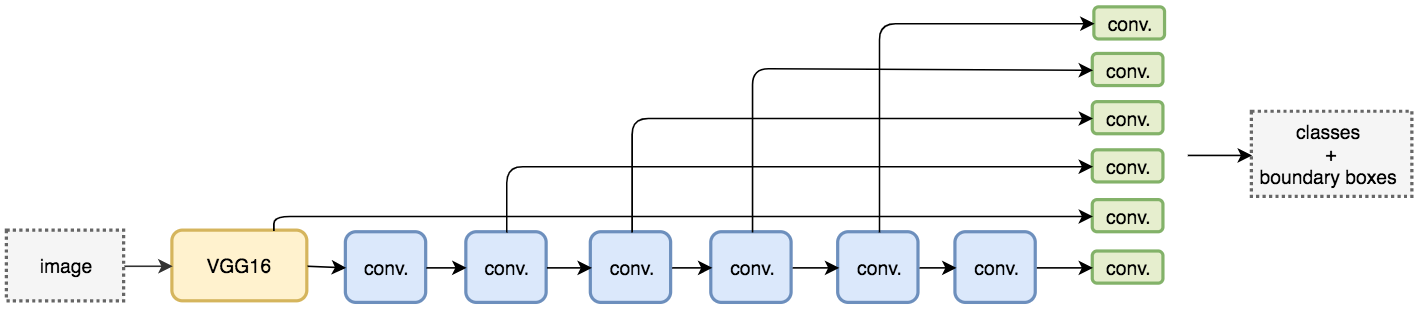
\includegraphics[width=1\textwidth]{vgg16-ssd}
    \caption[Example of the SSD architecture using VGG16 as its base network]{Example
    of the SSD architecture using VGG16 as its base network~\cite[cf.][]{Liu.2016}.
    \\\\
    Blue colored boxes represent the additional \glspl{convolutional layer} that are added to the base network.
    \\\\
    Green boxes represent the final additional \glspl{convolutional layer} that produce
    the classes- and \gls{bbox} predictions.}
    \label{fig:ssd-vgg}
\end{figure}
Then (as briefly addressed in \cref{subsect:default-boxes}), a set of
\glspl{convolutional layer} \(\mathbf{L}\) is chosen from the network (i.e.\
\(\mathbf{L}\subseteq \text{Network}\))\footnote{\label{foot:receptive}The motivation
behind choosing multiple layers \(\mathbf{L}\) from the network is as follows:
the \glspl{feature map} produced by the \glspl{convolutional layer} get smaller
with every additional layer. Colloquially speaking, the relationship between such
a small \gls{feature map} and the input image is, that one pixel within the small
\gls{feature map} is related to multiple pixels within the original input image.
Therefore, when looking at the \glspl{feature map} from subsequent
\glspl{convolutional layer}, one is looking at information that is extracted from
the image at different scales.

Making this logic concrete, in a larger \gls{feature map}, one pixel might contain
condensed information about objects like wheels or headlights, whereas in a smaller
\gls{feature map} one pixel might contain  condensed information about the entire
car. This concept is called the \textit{receptive field}~\cite[cf.][331\psq]{Goodfellow.2016}.}.

To produce class- and \gls{bbox} predictions, every chosen \glspl{layer} \(L\in \mathbf{L}\)
is fed into a final additional \gls{convolutional layer} (i.e.\ one additional
\gls{convolutional layer} per \gls{layer} in \(\mathbf{L}\), depicted green in \cref{fig:ssd-vgg}).

As discussed in \cref{subsect:default-boxes}, the model prediction is supposed
to be the quadruple \(o = \left(o^h, o^w, o^x, o^y\right)\). To enable also the
prediction of different object classes, \(c\) is appended to the quadruple
\(o\), where \(c\) is a one-hot encoded vector~\cite[cf.][35]{Murphy.2012} of all
classes\footnotemark.
The output size per chosen layer \(L\in \mathbf{L}\), with \gls{feature map} size
\(m\times n\) can be determined as \(m\times n\times \left(4 + \abs*{c}\right)\).

The output size of a 2D-\gls{convolutional layer} is the triplet
\(\left(\text{width}\times \text{height}\times \text{filter size}\right)\). Width
and height are calculated via \cref{eq:conv-output}, the filter size is chosen
without constraints.
\begin{equation}\label{eq:conv-output}
    W' = (W - F + 2P) \divslash S + 1
\end{equation}
where:
\begin{conditions}
    W & := & input size\\
    K & := & kernel size\\
    P & := & padding size\\
    S & := & stride size
\end{conditions}
To produce an output of size \(m\times n \times \left(4 + \abs*{c}\right)\),
kernel, padding, and stride sizes are therefore chosen \(K = 3, P = 1, S = 1\);
filter size is chosen as \(\left(4 + \abs*{c}\right)\).

This concludes the overall \gls{ssd} architecture.

\footnotetext{Actually, \(c\) is the one-hot encoded vector of all classes \(+1\).
This additional class is the \textit{no-object}-prediction. This is required because
obviously most areas within the image contain no classifiable object, and it is
desirable that the model is able to identify areas not containing an object.}

\subsection{Loss Function}
From previous subsections, a set of layers \(\mathbf{L}\) has been chosen from
the network \(\mathbf{L}\subseteq \text{Network}\). For the output (i.e.\ the
\gls{feature map}) of every such layer a set of default boxes \(D\in \mathbf{D}\)
has been generated. Also, for every image a set of \gls{gt} \glspl{bbox} \(B\) is
given from which the offsets \(O\) are computed following \cref{eq:offset-calc}
and \(o_{b,d}\) is the offset related to \gls{bbox} \mathvar{b} and default box
\mathvar{d}.
Next, a set of matching \gls{gt} \gls{bbox} offsets and default boxes is built in
\cref{eq:positives}:
\begin{align}
    \begin{split}\label{eq:positives}
        &\text{Let}\ \left(D\in \mathbf{D}\right)\land \left(d\in D\right)\land \left(b\in B\right)\\
        &\text{Then:}\\
        &\quad \text{Pos} = \left\{\left(d, o_{b,d}\right) \,\middle|\, \text{IoU}\left(d, b\right) > 0.5 \lor \forall{D'\in\mathbf{D}}\ldotp\nexists{d'\in{}D'}: \text{IoU}\left(d,b,\right) > \text{IoU}\left(d',b,\right)\right\}
    \end{split}
\end{align}
That is, \(\left(d,b\right)\) are added to Pos if their \gls{iou} is either greater than 0.5
or if no other default box (out of all default boxes over all layers) has a larger
\gls{iou}. The set of negative default boxes is then simply the complement as per
\cref{eq:negatives}:
\begin{equation}\label{eq:negatives}
    \text{Neg} = \left\{d \,\middle|\, \left(D\in \mathbf{D}\right)\land \left(d\in D\right)\land d \notin \text{Pos}\right\}
\end{equation}
From the model architecture \cref{subsect:SSD Architecture} it becomes apparent,
that the \(\abs*{\text{Negatives}} \gg \abs*{\text{Positives}}\). To prevent
overfitting~\cite[cf.][111\psqq]{Goodfellow.2016} the model, for example s.t.\
it detects only negatives, the \emph{amount} of negatives is pruned\footnotemark{}
to be only three times greater than the number of positives.
\footnotetext{This process is also called hard negatives mining, please
confer~\cite{Liu.2016}.}
Therefore, the set of negatives is ordered by their class confidence score\footnotemark{} and then cut off at index
\(\left\lfloor 3*\abs*{Positives}\right\rfloor\).

\footnotetext{In order to spare the reader, the exact derivation of the relation
which specifies the order required for pruning is omitted.}

Finally, the loss is the weighted sum of the confidence loss (\cref{eq:conf-loss}) and the
location loss \cref{eq:loc-loss}. Let \(\mathds{1}_{b}^p = \{0, 1\}\) indicate, that
\gls{gt} \gls{bbox} \mathvar{b} is of class \mathvar{p}.
The confidence loss 
\begin{alignat}{3}
    \label{eq:conf-loss}&L_{\text{conf}}(l)     &=& - \sum_{p=1}^{\alphaAbs{C}} \left[ \sum_{\left(d,o\right)\in \text{Pos}} \mathds{1}_{o}^p * \log\left(\sigma\left(l_d^p\right)\right)\right] - \sum_{i\in \text{Neg}}\log\left(\sigma\left(l_d^0\right)\right)\\
    \label{eq:loc-loss}&L_{\text{loc}}(l)       &=& \sum_{\left(d,o\right)\in \text{Pos}} \sum_{m\in \left\{ h,w,x,y \right\}} \operatorname{smooth_{L1}}\left(l_d^m - o_d^m\right)\\
    \label{eq:softmax}&\sigma\left(l_d^p\right) &=& \frac{\exp{\left(l_d^p\right)}}{\sum_{p'}{\exp\left(l_d^{p'}\right)}}
\end{alignat}
where:
\begin{conditions}
    C &:= & is the set of all n-classes \(\left[1, n\right]\) without the \textit{no-object} class \(0\)\\
    l &:= & Prediction produced by the model\\
    l_d^p &:= & Prediction associated with default box \mathvar{d} and class \mathvar{p}\\
    l_d^m &:= & Prediction associated with default box \mathvar{d} and dimension \(m\in \left\{h,w,x,y\right\}\)\\
    o_d^m &:= & Offset (see \cref{eq:offset-calc}) associated with default box \mathvar{d} and dimension \(m\in \left\{h,w,x,y\right\}\)


\end{conditions}
The final loss is now given in \cref{eq:loss}.
\begin{equation}\label{eq:loss}
    L(l) =
    \begin{cases}
        \frac{1}{\alphaAbs{\mathrm{Pos}}}\left(L_{\text{conf}(l)} + \alpha L_{\text{loc}}(l)\right),& \text{if }  \geq 1\\
        0, & \text{otherwise}
    \end{cases}
\end{equation}
